\section{Source Seeking: Collaboration with Peter Paulsen}
%%%%%%%%%%%%%%%%%%%%%%%%%%%%%%%%%%%%%%%%%%%%%%%%%%%%%%%%%%%%%%%%%%%%%
\subsection{Problem}
%%%%%%%%%%%%%%%%%%%%%%%%%%%%%%%%%%%%%%%%%%%%%%%%%%%%%%%%%%%%%%%%%%%%%
\begin{frame}{Source seeking problem}
%	\begin{minipage}{0.45\textwidth}	
%		%\hspace{0.4cm}		
%%		\begin{figure}
%%			\includegraphics[width=\textwidth]{figures/fukushima_disaster_final.png}
%%			%\caption{Fukushima Disaster}
%%			%\label{fig:fukushima_disaster}
%%		\end{figure}
%	\end{minipage}
%	\hspace{0.05cm}
%	\begin{minipage}{0.45\textwidth}
%%		\begin{figure}
%%			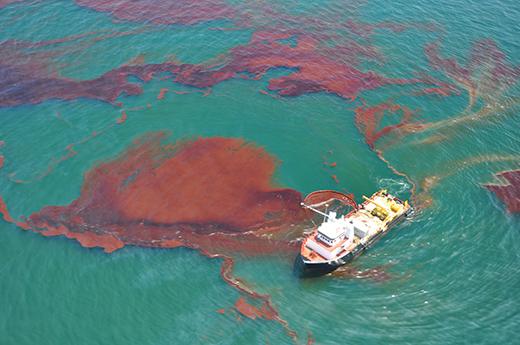
\includegraphics[width=\textwidth]{figures/oil_spill.png}
%%			%\caption{Oil Spills}
%%			%\label{fig:oilspills}
%%		\end{figure}
%	\end{minipage}
\vspace{0.5cm}
\textbf{Idea at the core:}
\begin{itemize}
	\item Disaster striken areas could be dangerous and potentially life threatening for humans 
	\item Deploy a swarm of autonomous robots with sensing and communication capabilities to locate the source of accident.
\end{itemize}
\end{frame}
%%%%%%%%%%%%%%%%%%%%%%%%%%%%%%%%%%%%%%%%%%%%%%%%%%%%%%%%%%%%%%%%%%%%%
\begin{frame}{Capabilities of a single agent (Robot)}
\begin{itemize}
	\item Position information based on an indoor positioning system (can be relaxed to only distance measurements)
	\item Peer to peer communication and computation capabilites onboard
	\item Pretend to measure the strength of a virtual scalar field based on the current location
\end{itemize}		
\end{frame}
%%%%%%%%%%%%%%%%%%%%%%%%%%%%%%%%%%%%%%%%%%%%%%%%%%%%%%%%%%%%%%%%%%%%%
\begin{frame}{Source seeking problem as optimization}
\begin{itemize}
	\item Look at the source seeking problem as an minimization problem
	\item Momentum methods\footnote{Polyak,1964} have been used in optimization to speed up or dampen the oscillations
	\item Naturally have momentum of the robots   
	\item For theoretical analysis: Use continuous-time versions of optimization methods to study the assymptotic properties\footnote{Redont et al., 2002} 
\end{itemize}
\end{frame}
%%%%%%%%%%%%%%%%%%%%%%%%%%%%%%%%%%%%%%%%%%%%%%%%%%%%%%%%%%%%%%%%%%%%%
\subsection{Theory}
%%%%%%%%%%%%%%%%%%%%%%%%%%%%%%%%%%%%%%%%%%%%%%%%%%%%%%%%%%%%%%%%%%%%%
\begin{frame}{Continuous-time steepest descent with momentum}
\begin{itemize}
\item Consider the problem of minimizing a differentiable $f:\mathbb{R}^n\rightarrow \mathbb{R}$
\pause
\item The steepest descent iteration is
\begin{equation}
x_{k+1}=x_k - \alpha \nabla f(x_k)
\end{equation}
\pause
\item The continuous-time version of the steepest descent dynamics 
\begin{equation}
\dot{x}= - \nabla f(x_k)
\end{equation}
\pause
\item The continuous-time version of the steepest descent dynamics with momentum (also known as the heavy ball method with friction) 
\begin{equation}
m\ddot{x}+ \dot{x}= - \nabla f(x_k)
\end{equation}
\end{itemize}
\end{frame}
%%%%%%%%%%%%%%%%%%%%%%%%%%%%%%%%%%%%%%%%%%%%%%%%%%%%%%%%%%%%%%%%%%%%%
\begin{frame}{Continuous-time Newton with momentum}
\begin{itemize}
	\item Consider the problem of minimizing a twice-differentiable, strongly convex $f:\mathbb{R}^n\rightarrow \mathbb{R}$
	\pause
	\item The Newton iteration is
	\begin{equation}
	x_{k+1}=x_k - \alpha\nabla^2f(x_k)^{-1} \nabla f(x_k)
	\end{equation}
	\pause
	\item The continuous-time version of these dynamics can be represented as
	\begin{equation}
	\nabla^2f(x_k)\dot{x}= - \nabla f(x_k)
	\end{equation}
	\pause
	\item Adding momentum to these dynamics gives  
	\begin{equation}
	m\ddot{x}+ \nabla^2f(x_k)\dot{x}= - \nabla f(x_k)
	\end{equation}
\end{itemize}
\pause
Defining the velocity variable $v$, the dyanmics can be written as 
\begin{equation} \label{eqn: second_order_newton_cont_time}
\begin{split}
\Dot{x}&=v\\
\Dot{v}&=-k_1\nabla^2 f(x) v -k_2 \nabla f(x), 
\end{split}
\end{equation}
\end{frame}
%%%%%%%%%%%%%%%%%%%%%%%%%%%%%%%%%%%%%%%%%%%%%%%%%%%%%%%%%%%%%%%%%%%%%
\begin{frame}{Flocking and schooling in nature}

\begin{minipage}{0.45\textwidth}	
	%\hspace{0.4cm}	
	\begin{figure}
		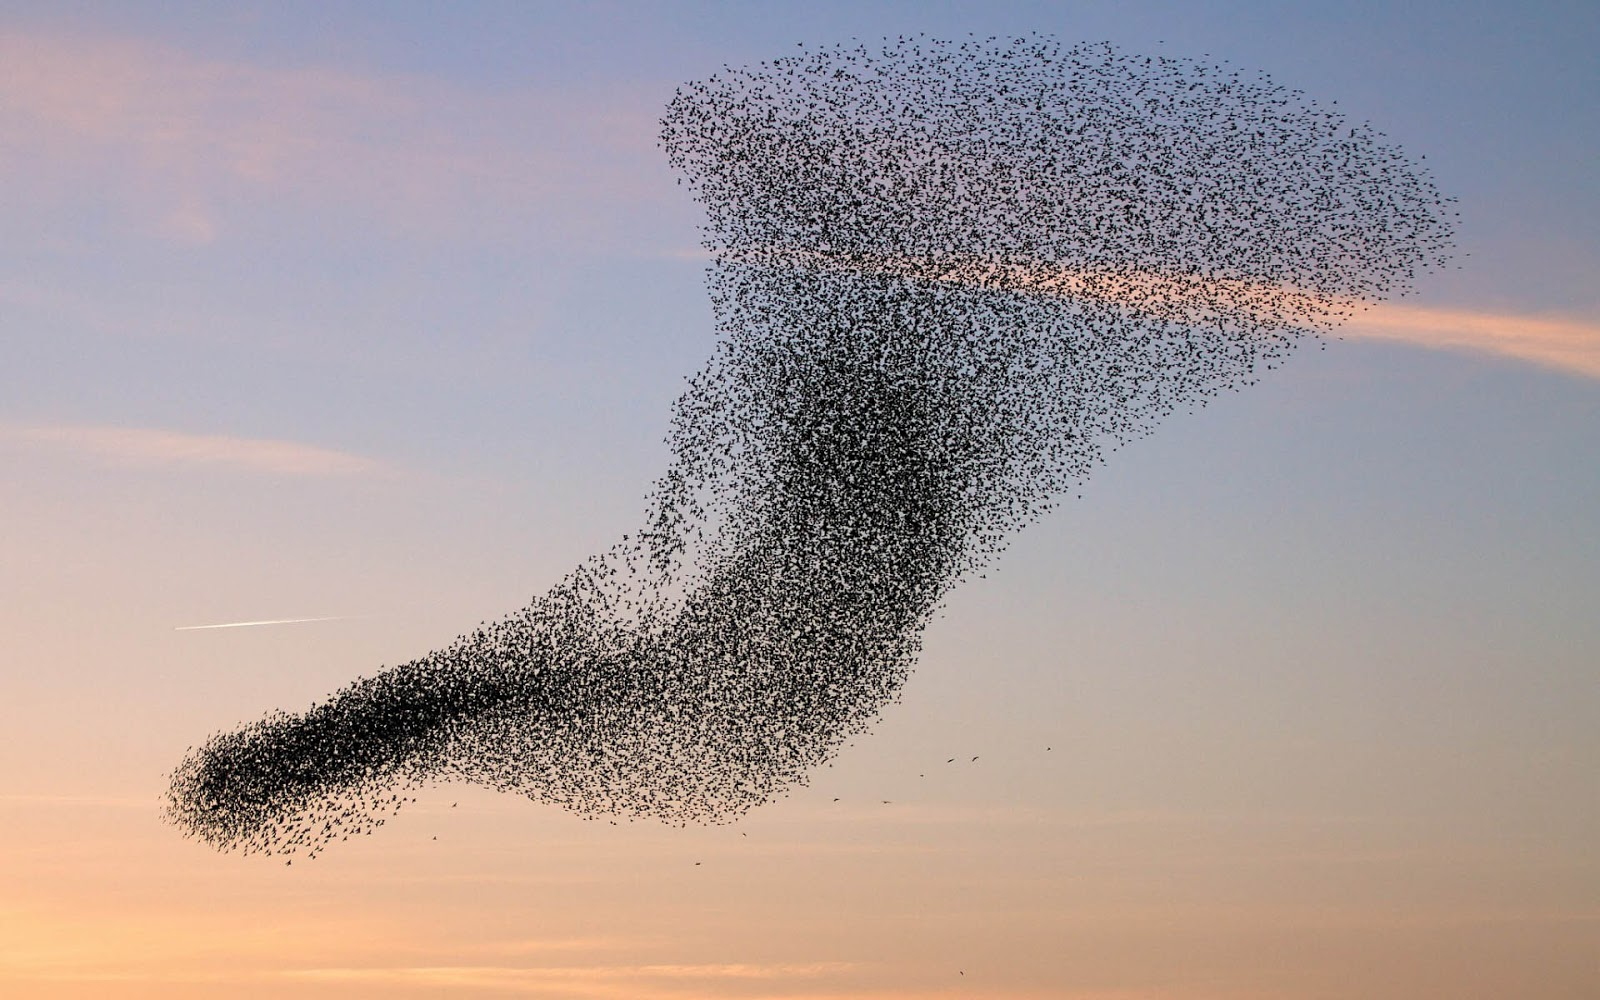
\includegraphics[width=\textwidth]{figures/flock_of_birds.jpg}
		%\caption{Fukushima Disaster}
		%\label{fig:flock_of_birds}
	\end{figure}
\end{minipage}
\hspace{0.05cm}
\begin{minipage}{0.45\textwidth}	
	\begin{figure}
		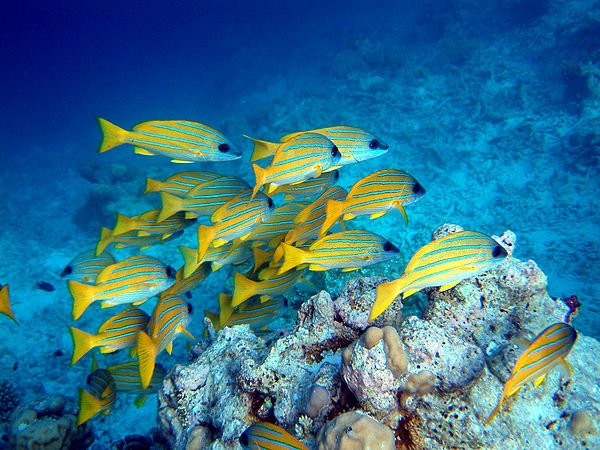
\includegraphics[width=\textwidth]{figures/schooling_fish.jpg}
		%\caption{Oil Spills}
		%\label{fig:schools_of_fish}
	\end{figure}
\end{minipage}
\begin{itemize}	
	\item The precise rules that these animals use are not known
	\item Particle-based flocking seems to be an effective approach to model such behavior
	\item In 1987, Reynold was working on animating flocking behavior where he proposed three rule
	\begin{itemize}
		\item Cohesion: Attempt to stay close to nearby neighbors
		\item Separation: Avoid collisions with nearby flockmates
		\item Alignment: attempt to match velocities with nearby flockmates
	\end{itemize}
\end{itemize}
\end{frame}
%%%%%%%%%%%%%%%%%%%%%%%%%%%%%%%%%%%%%%%%%%%%%%%%%%%%%%%%%%%%%%%%%%%%%
\begin{frame}{Flocking dynamics}
\begin{itemize}
	\item Every particle interacts with every other particle based on an interaction field $V$ which depends only on the distance between them
	\item An example of a potential field is the gravitational field $V(z)=\frac{mMG}{||z||}$
	\item Flocking dynamics\footnote{Olfati-Saber, 2004}:
	\begin{equation*}
	\begin{split}
	\Dot{q}&=p\\
	\Dot{p}&=-\nabla V(q)-\hat{L}(q)p -cp 
	\end{split}
	\end{equation*}
\end{itemize}
\end{frame}
%%%%%%%%%%%%%%%%%%%%%%%%%%%%%%%%%%%%%%%%%%%%%%%%%%%%%%%%%%%%%%%%%%%%%
\begin{frame}{Flocking towards the source}
\begin{itemize}
\item Consider now an underlying source field $\psi:\mathbf{R}^m \xrightarrow{} \mathbf{R}$ which is smooth enough and convex.
\item Add a forcing term to the flocking dynamics motivated from the discussion on optimization
\item Flocking dynamics with source-seeking:
\begin{equation*}
\begin{split}
\Dot{q}&=p\\
\Dot{p}&=-\nabla V(q)-\hat{L}(q)p -cp\textcolor{red}{-k_1\nabla^2 \Psi(q) p -k_2 \nabla \Psi(q)}
\end{split}
\end{equation*}
\end{itemize}
\end{frame}
%%%%%%%%%%%%%%%%%%%%%%%%%%%%%%%%%%%%%%%%%%%%%%%%%%%%%%%%%%%%%%%%%%%%%
\begin{frame}{Stability(Convergence) Analysis}
	Flocking dynamics with source-seeking:
	\begin{equation*}
	\begin{split}
	\Dot{q}&=p\\
	\Dot{p}&=-\nabla V(q)-\hat{L}(q)p -cp\textcolor{red}{-k_1\nabla^2 \Psi(q) p -k_2 \nabla \Psi(q)}
	\end{split}
	\end{equation*}
\textbf{Theorem 5} For smooth enough strictly convex fields $\psi:\mathbf{R}^m \xrightarrow{} \mathbf{R}$ with a single minima, the above flocking dynamics is stable i.e the trajectories remain bounded. Moreover, for all initial conditions $(q(0),p(0))$, the trajectories converge asymptotically to the set $$\mathcal{W}:=\{(q^*,0)|\nabla V (q^*)+ \Psi(q^*) = 0 \}.$$

Additionally, if the field $\psi:\mathbf{R}^m \xrightarrow{} \mathbf{R}$ is quadratic and has a single unique minimum located at $q_s$, we have that $\lim_{t\rightarrow \infty}q_c(t)=q_s$
\end{frame}
%%%%%%%%%%%%%%%%%%%%%%%%%%%%%%%%%%%%%%%%%%%%%%%%%%%%%%%%%%%%%%%%%%%%%
\begin{frame}{Stability(Convergence) Analysis}
\textbf{Sketch of the proof:}
	\begin{itemize}
		\item Define the energy function
		\begin{equation*}\label{eqn: energy function}
		E(t):= V(q(t)) + k_2\Psi(q(t)) + \frac{1}{2}p(t)^Tp(t).
		\end{equation*}
		\pause
		\item Differentiating w.r.t time, 
		\begin{equation*}
		\begin{split}
		\dot{E}&= (\nabla V(q) + k_2\nabla \Psi(q))^T\dot{q} + p^T\dot{p} \\
		&=-p^T(\hat{L}(q)+cI+k_1\nabla^2\Psi(q))p\\
		&\leq 0.
		\end{split}
		\end{equation*}
		\pause
		\item $E(t)\leq E(0) ~\forall t\geq0$ implies the boundedness of trajectories
		\pause
		\item  $\dot{E}=0 \iff p=0$. Thus, LaSalle's invariance principle $\implies$ that the trajectories converge to the largest invariant set contained in $\mathcal{W}:=\{(q^*,0)|\nabla V (q^*)+ \nabla \Psi(q^*) = 0 \}$
	\end{itemize}
\end{frame}
%%%%%%%%%%%%%%%%%%%%%%%%%%%%%%%%%%%%%%%%%%%%%%%%%%%%%%%%%%%%%%%%%%%%%
\begin{frame}{Stability(Convergence) Analysis}
	\textbf{Sketch of the proof(ctd):}
	\begin{itemize}
		\item To characterize the equilibrium, we write the dynamics of the center of mass
		\begin{equation} \label{eqn: COM flocking dynamics}
		\begin{split}
		\Dot{q}_c&=p_c\\
		\Dot{p}_c&=-cp_c-\frac{1}{N}(\mathbf{1}_N\otimes I_m)^T(k_1\nabla^2\Psi(q) p +k_2 \nabla\Psi(q)) 
		\end{split}
		\end{equation}
		\pause
		\item $\lim_{t\rightarrow \infty}p(t)=0 \implies \lim_{t\rightarrow \infty}p_c(t)=0$
		\pause
		\item For quadratic $\psi(q)=\frac{1}{2}q^THq+g^Tq+c_0$, with $H\succ 0$, the source is the unique solution to $Hq_s+g=0$
		\pause
		\item At equilibrium $q^*$, 
		\begin{equation*}
		\begin{split}
		\frac{1}{N}\sum_{i=1}^{N}\nabla\psi(q_i^*)&=0 \iff \textnormal{i.e } H(\frac{1}{N}\sum_{i=1}^{N}q_i^*)+g=0\\
		\textnormal{i. e  } Hq_c^*+g&=0 \iff q_c^*=q_s
		\end{split}	
		\end{equation*}
	\end{itemize}
\end{frame}
%%%%%%%%%%%%%%%%%%%%%%%%%%%%%%%%%%%%%%%%%%%%%%%%%%%%%%%%%%%%%%%%%%%%%
\subsection{Experiments}
%%%%%%%%%%%%%%%%%%%%%%%%%%%%%%%%%%%%%%%%%%%%%%%%%%%%%%%%%%%%%%%%%%%%%
\begin{frame}{Towards implementation: Local velocity controller}
\begin{figure}[h!]
	\tikzstyle{block} = [draw, rectangle, 
    minimum height=3em, minimum width=6em]
\tikzstyle{sum} = [draw,  circle, node distance=1cm]
\tikzstyle{input} = [coordinate]
\tikzstyle{output} = [coordinate]
\tikzstyle{pinstyle} = [pin edge={to-,thin,black}]

% The block diagram code is probably more verbose than necessary
%\begin{tikzpicture}[auto, node distance=2cm,>=latex']
%    % We start by placing the blocks
%    \node [input, name=input] {};
%    \node [sum, right of=input] (sum) {};
%    \node [block, right of=sum] (controller) {Controller};
%    \node [block, right of=controller, pin={[pinstyle]above:Disturbances},
%            node distance=3cm] (system) {System};
%    % We draw an edge between the controller and system block to 
%    % calculate the coordinate u. We need it to place the measurement block. 
%    \draw [->] (controller) -- node[name=u] {$u$} (system);
%    \node [output, right of=system] (output) {};
%    \node [block, below of=u] (measurements) {Measurements};
%
%    % Once the nodes are placed, connecting them is easy. 
%    \draw [draw,->] (input) -- node {$r$} (sum);
%    \draw [->] (sum) -- node {$e$} (controller);
%    \draw [->] (system) -- node [name=y] {$y$}(output);
%    \draw [->] (y) |- (measurements);
%    \draw [->] (measurements) -| node[pos=0.99] {$-$} 
%        node [near end] {$y_m$} (sum);
%\end{tikzpicture}

\begin{tikzpicture}[auto, node distance=2cm,>=latex']
% We start by placing the blocks
\node [input, name=input] {};
\node [block, right of=input,pin={[pinstyle]above:$\Psi(q)$},node distance=2.5cm](Flockcontrol) {$u=-\nabla V-(\hat{L}+cI)p + f_{\gamma} $};
\node [block, right of=Flockcontrol,node distance=3cm,minimum height=1em,minimum width=2em](integrator) {$\frac{1}{s}$};
\node [block, right of=integrator,node distance=2cm,minimum height=2.5em,minimum width=3em](velocityloop) {$G_{\textnormal{vel}}$};
\node [output, right of=velocityloop,node distance=1cm](output) {};
\node [block, below of=integrator,node distance=2cm](network) {Network};
% Once the nodes are placed, connecting them is easy. 
\draw [draw,->] (input) -- node {} (Flockcontrol);
\draw [draw,->] (Flockcontrol) -- node {} (integrator);
\draw [draw,->] (integrator) -- node {$p_{\textnormal{des}}$} (velocityloop);
\draw [draw,->] (velocityloop) -- node[name=outmid] {$\begin{bmatrix}q\\p\end{bmatrix}$} (output);
\draw [->] (outmid) |- (network);
\draw [-] (network) -| (input);
\end{tikzpicture}
	\caption{Control Architecture}
	\label{fig:control_arch}	
\end{figure}
\begin{itemize}
	\item $G_{\textnormal{vel}}$ is the closed loop velocity tracking dynamics
	\item The velocity controller is fast enough $\implies$ approximate $G_{\textnormal{vel}}$ by single integrator dynamics.
\end{itemize}
\end{frame}
%%%%%%%%%%%%%%%%%%%%%%%%%%%%%%%%%%%%%%%%%%%%%%%%%%%%%%%%%%%%%%%%%%%%%
\begin{frame}{Towards implementation: Gradient and hessian information}
%	\begin{figure}[h!]	
%		\includegraphics[width=6cm]{figures/error_direction_Noise.png}
%		%\caption{Histograms of errors (in angles) between the estimated and true gradient direction and modified Newton step direction when the field measurements are corrupted}
%		\label{fig:direction_errors_noise}
%	\end{figure}
\begin{itemize}
	\item Corrupt the field strength measurement by +/- 5 percent of the field strength. 
	\item Estimate gradient by collecting local data and solving a least squares problem
	\item Estimate the hessian by collecting data from neighbors and solving another least squares problem
\end{itemize}
\end{frame}
%%%%%%%%%%%%%%%%%%%%%%%%%%%%%%%%%%%%%%%%%%%%%%%%%%%%%%%%%%%%%%%%%%%%%
\begin{frame}{Towards implementation: Hueristic for non-convex fields}
\begin{itemize}
	\item Use gradient information until the estimated hessian is positive definite
	\item Switch between newton and steepest descent 
	\item One could use Levenberg–Marquardt type methods (future work)
\end{itemize}
\end{frame}
%%%%%%%%%%%%%%%%%%%%%%%%%%%%%%%%%%%%%%%%%%%%%%%%%%%%%%%%%%%%%%%%%%%%%%
%\begin{frame}{Experimental Results: Quadratic field(Video)}
%\includemedia[
%activate=pageopen,
%width=300pt,height=200pt,
%addresource=animations/OBLIQUE_quadratic_mod_newton_Fig_4.mp4,
%flashvars={%
%	src=figures/noObstacle.mp4      % same path as in addresource!
%	%&scaleMode=stretch % removes black bars
%	&autoPlay=true      % optional configuration
%	&loop=true          % variables
%}
%]{}{StrobeMediaPlayback.swf}
%\end{frame}
%%%%%%%%%%%%%%%%%%%%%%%%%%%%%%%%%%%%%%%%%%%%%%%%%%%%%%%%%%%%%%%%%%%%%%
%\begin{frame}{Experimental Results: Quadratic field(Animation)}
%
%		\includemedia[
%		activate=pageopen,
%		width=300pt,height=200pt,
%		addresource=animations/convex.mp4,
%		flashvars={%
%			src=figures/noObstacle.mp4      % same path as in addresource!
%			%&scaleMode=stretch % removes black bars
%			&autoPlay=true      % optional configuration
%			&loop=true          % variables
%		}
%		]{}{StrobeMediaPlayback.swf}
%
%\end{frame}
%%%%%%%%%%%%%%%%%%%%%%%%%%%%%%%%%%%%%%%%%%%%%%%%%%%%%%%%%%%%%%%%%%%%%%
%\begin{frame}{Experimental Results: Log-Convex quadratic field (Video)}
%		\includemedia[
%		activate=pagevisible,
%		width=300pt,height=200pt,
%		addresource=animations/OBLIQUEVIEW__log_convex_mod_newton_Fig_5.mp4,
%		flashvars={%
%			src=figures/noObstacle.mp4      % same path as in addresource!
%			%&scaleMode=stretch % removes black bars
%			&autoPlay=true      % optional configuration
%			&loop=true          % variables
%		}
%		]{}{StrobeMediaPlayback.swf}
%\end{frame}
%%%%%%%%%%%%%%%%%%%%%%%%%%%%%%%%%%%%%%%%%%%%%%%%%%%%%%%%%%%%%%%%%%%%%%
%\begin{frame}{Experimental Results: Log-Convex quadratic field (Animation)}
%	\includemedia[
%	activate=pagevisible,
%	width=300pt,height=200pt,
%	addresource=animations/quasiConvex.mp4,
%	flashvars={%
%		src=figures/noObstacle.mp4      % same path as in addresource!
%		%&scaleMode=stretch % removes black bars
%		&autoPlay=true      % optional configuration
%		&loop=true          % variables
%	}
%	]{}{StrobeMediaPlayback.swf}
%\end{frame}
%%%%%%%%%%%%%%%%%%%%%%%%%%%%%%%%%%%%%%%%%%%%%%%%%%%%%%%%%%%%%%%%%%%%%%
%\begin{frame}{Experimental Results: Field with multiple minima (Video)}
%	\includemedia[
%	activate=pageopen,
%	width=300pt,height=200pt,
%	addresource=animations/2 minima mod Newton noise.mp4,
%	flashvars={%
%		src=figures/noObstacle.mp4      % same path as in addresource!
%		%&scaleMode=stretch % removes black bars
%		&autoPlay=true      % optional configuration
%		&loop=true          % variables
%	}
%	]{}{StrobeMediaPlayback.swf}
%\end{frame}
%%%%%%%%%%%%%%%%%%%%%%%%%%%%%%%%%%%%%%%%%%%%%%%%%%%%%%%%%%%%%%%%%%%%%%
%\begin{frame}{Experimental Results: Field with multiple minima (Animation)}
%	\includemedia[
%	activate=pageopen,
%	width=300pt,height=200pt,
%	addresource=animations/2minima.mp4,
%	flashvars={%
%		src=figures/noObstacle.mp4      % same path as in addresource!
%		%&scaleMode=stretch % removes black bars
%		&autoPlay=true      % optional configuration
%		&loop=true          % variables
%	}
%	]{}{StrobeMediaPlayback.swf}
%\end{frame}
%%%%%%%%%%%%%%%%%%%%%%%%%%%%%%%%%%%%%%%%%%%%%%%%%%%%%%%%%%%%%%%%%%%%%